\nsection{Problem 4 - (Combinatorial optimization)}
 In this problem we will consider a logistics problem. Assume that you work in a company which want to distribute their product to 20 cities, starting from its home city. In the file \texttt{optimaltransport.dat} you will find the locations of all 21 cities the distances between the cities is the time it takes to travel between them. The first city in the file is the home city. We want to find the loop which reduces the traveling time going from the home city, cycling through all cities and returning to the home city. You can modify the scripts found on the home page of the course to solve the problem.
\nssection{a.)}
\emph{Write an optimization using simulated annealing to find the optimal solution. Define your neighborhood using mathematical notation. Define your cooling schedule. Argue that your proposed algorithm can reach all possible states.} \spaze
\textbf{Solution:} \spaze
In this implementation we have defined the neighbourhood 
\begin{align*}
    \mathcal{N}(\boldsymbol{\theta}) = \bl\boldsymbol{\theta}^{*} ; \exists \ i,j \ \text{such that} \ \boldsymbol{\theta}_{i}^{*} = \boldsymbol{\theta}_j, \boldsymbol{\theta}_{j}^{*} = \boldsymbol{\theta}_i \ \land \ \boldsymbol{\theta}_{k}^{*} = \boldsymbol{\theta}_{k}, \forall k \neq i,j  \br
\end{align*}
which describes the action of swapping or switching to elements/entries in a sequence. For our problem this simply states the action of swapping to towns/cities in our heuristic. More rigidly, we could also define it as follows: \vspace{2mm}\\ 
Let \( \boldsymbol{\theta} \) be the tour represented as an ordered sequence of cities: \( \boldsymbol{\theta} = (t_1, t_2, \ldots, t_n) \), where \( t_i \) represents the \( i \)-th town in the tour.

The neighborhood \( \mathcal{N}(\boldsymbol{\theta}) \) of tour \( \boldsymbol{\theta} \) obtained by swapping cities \( i \) and \( j \) is defined as:

\[ \mathcal{N}(\boldsymbol{\theta}) = \{\boldsymbol{\theta}^{*} \mid \boldsymbol{\theta}^{*} \text{ is obtained by swapping towns } i \text{ and } j \text{ in } \boldsymbol{\theta} \} \]
Which in more syntactic language means:

\[ \mathcal{N}(\boldsymbol{\theta}) = \{\boldsymbol{\theta}^{*} \mid \boldsymbol{\theta}^{*} = (t_1, \ldots, t_{i-1}, t_j, t_{i+1}, \ldots, t_{j-1}, t_i, t_{j+1}, \ldots, t_n)\} \]

where \( \boldsymbol{\theta}^{*} \) is a permutation of the original tour \( \boldsymbol{\theta} \) with cities \( i \) and \( j \) swapped. 

The algorithm explores all possible states because it can move between any two tours by swapping adjacent cities. This connected structure ensures that every potential tour configuration can be constructed in a finite number of steps.

The code of the implementation can be found in Appendix \ref{appendix:b}, from code lisitings (\ref{lst:simul_anneal}) and produces the following plots 
\begin{figure}[H]
  \centering
  \begin{subfigure}{0.48\textwidth}
    \centering
    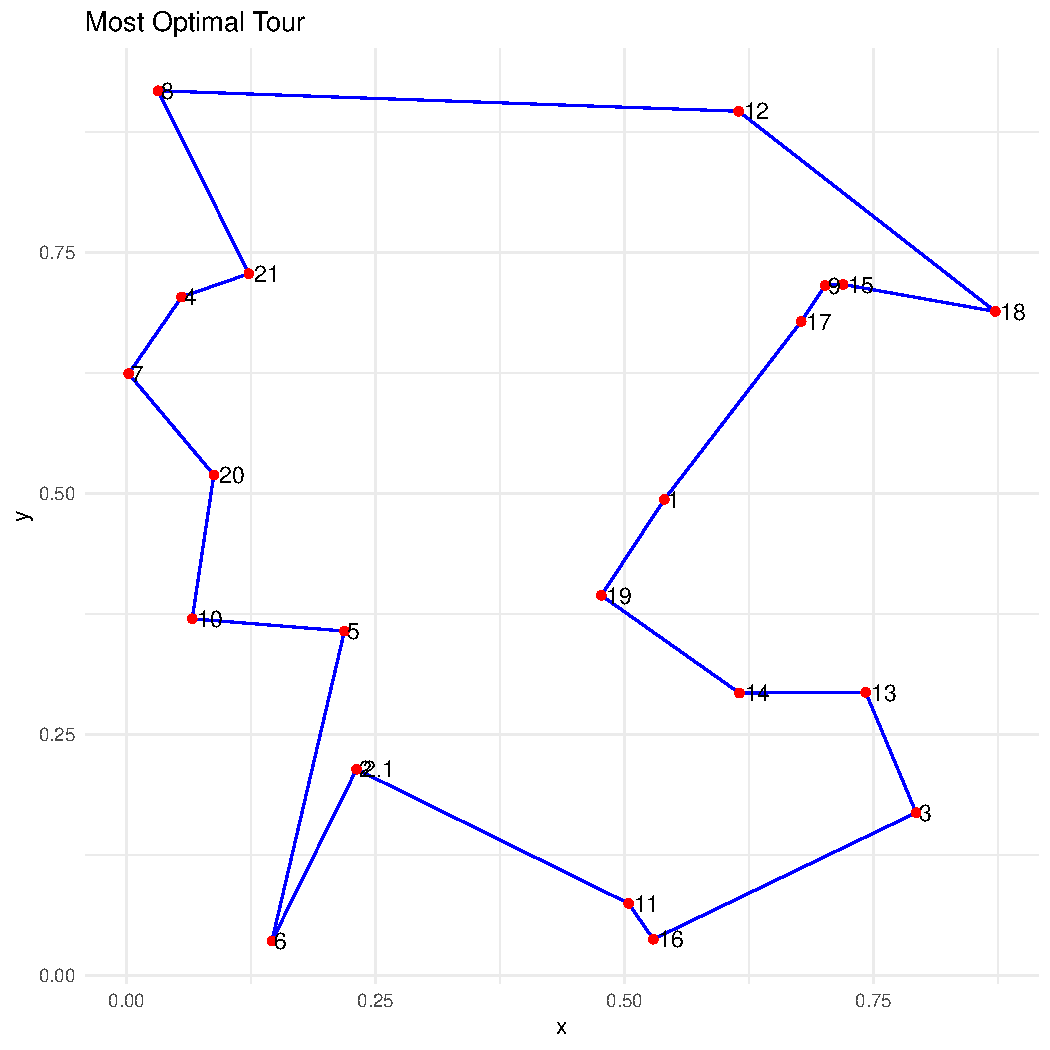
\includegraphics[width=\linewidth]{Images/Figures_Exercise_4/opt_annealing.pdf} % Replace with your first image file name
    \caption{}
    \label{fig:opt_annealing}
  \end{subfigure}
  \hfill
  \begin{subfigure}{0.48\textwidth}
    \centering
    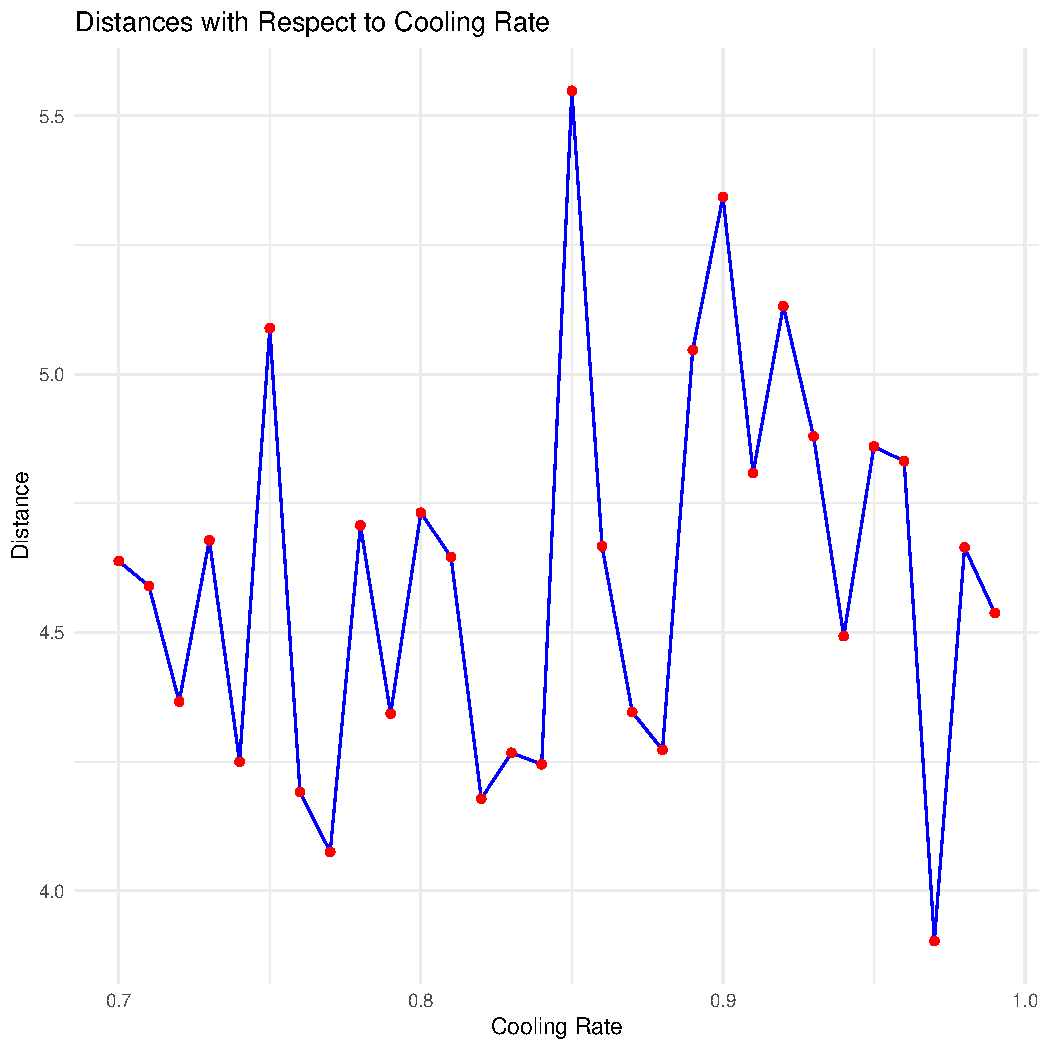
\includegraphics[width=\linewidth]{Images/Figures_Exercise_4/opt_cooling.pdf} % Replace with your second image file name
    \caption{}
    \label{fig:opt_cooling}
  \end{subfigure}
  \caption{Plots of the most optimal tour and cooling rate for the latest run.}
  \label{fig:annealing_plots}
\end{figure}
where the all time best tour $\boldsymbol{\theta}^{b}$ gave
\begin{align*}
    &\boldsymbol{\theta}^{b} = \bl 17, 9, 15, 18, 12, 8, 21, 4, 7, 20, 10, 5, 2, 6, 11, 16, 3, 13, 14, 19, 1 \br \\[5pt] 
    &\text{dist}( \boldsymbol{\theta}^{b}) =  3.770697 \\[5pt]
    &\alpha = 0.77 \quad \text{(Cooling rate)}
\end{align*}
\nssection{b.)}
\emph{Implement also a TABU search for the optimal path. In what way does both the simulated annealing and the TABU algorithm differ from a steepest decent algorithm?} \spaze 
\textbf{Solution:} \spaze
The code of the implementation can be found in Appendix \ref{appendix:b}, from code lisitings (\ref{lst:tabu}) and produces the following plots 
\begin{figure}[H]
  \centering
  \begin{subfigure}{0.49\textwidth}
    \centering
    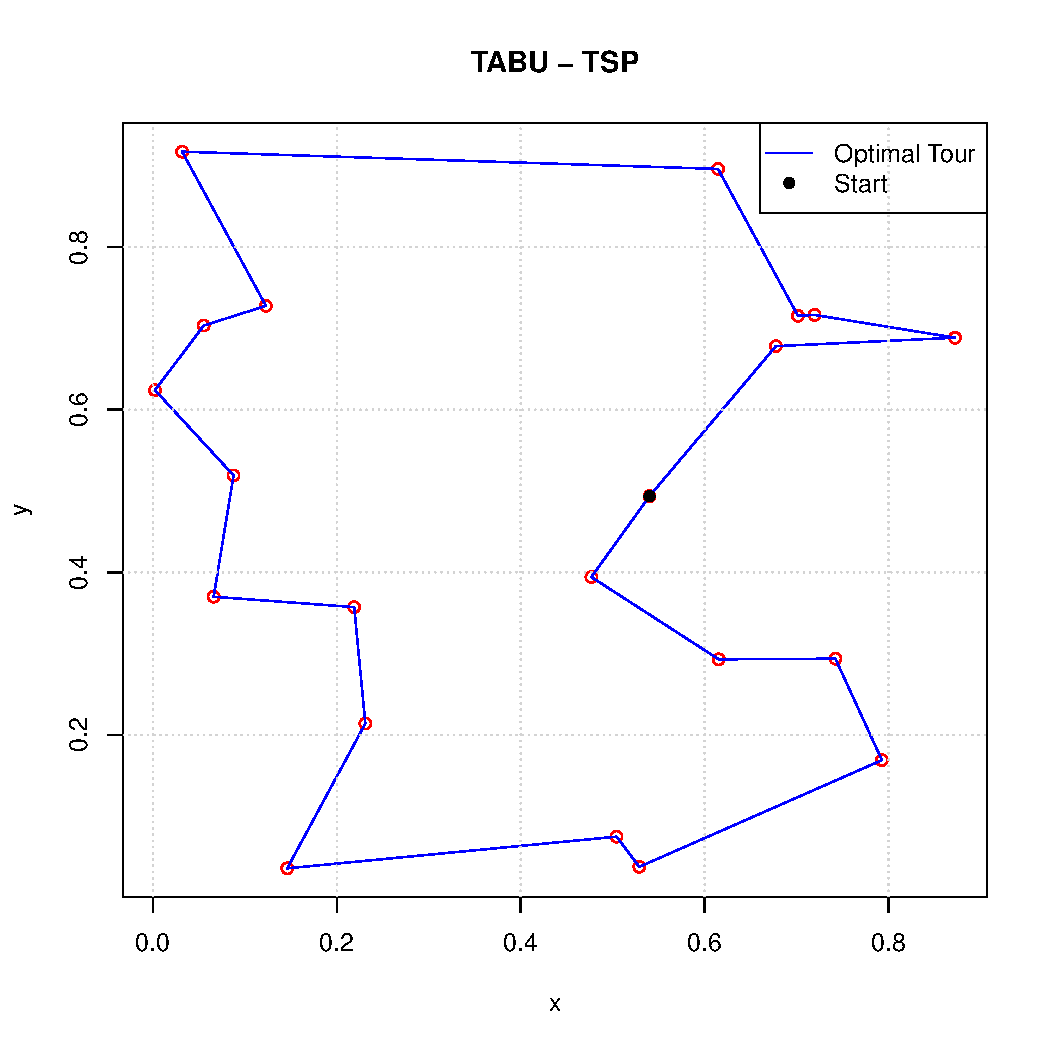
\includegraphics[width=\linewidth]{Images/Figures_Exercise_4/opt_tabu.pdf} % Replace with your first image file name
    \caption{}
    \label{fig:opt_tabu}
  \end{subfigure}
  \hfill
  \begin{subfigure}{0.49\textwidth}
    \centering
    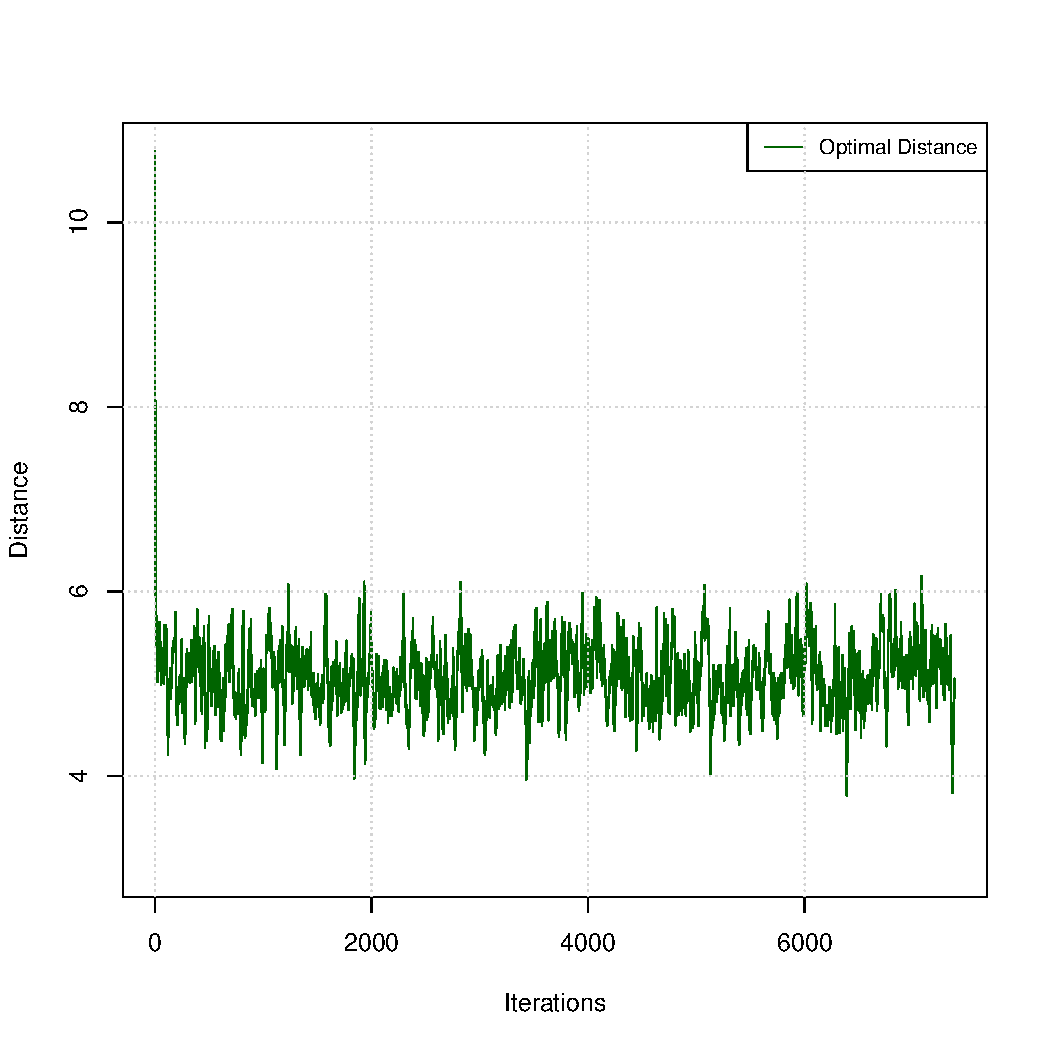
\includegraphics[width=\linewidth]{Images/Figures_Exercise_4/distance_iter.pdf} % Replace with your second image file name
    \caption{}
    \label{fig:opt_iter}
  \end{subfigure}
  \caption{Plots of the most optimal tour and evolution of distance with respect to iterations.}
  \label{fig:annealing}
\end{figure}
where the all time best tour $\boldsymbol{\theta}^{b}$ gave
\begin{align*}
    &\boldsymbol{\theta}^{b} = \bl 1, 14, 13, 3, 16, 11, 6, 2, 5, 7, 4, 21, 12, 9, 8, 15, 18, 10, 17, 20, 19 \br \\[5pt] 
    &\text{dist}( \boldsymbol{\theta}^{b}) =   3.581809 
\end{align*}
Simulated Annealing (SA) and Tabu Search (TS) algorithms differ from steepest descent by prioritizing exploration over exploitation. Steepest descent follows a determined search where it solely relies on the local information of the gradient. In contrast, SA and TS adopt more exploratory rules, therefore inclined to observe new territories in the solution space. \spaze
Mathematically, steepest descent iterates through solutions following the gradient direction  \( \nabla f(x_n) \) to minimize the objective function \( f(x) \). SA introduces randomness, with the probability of accepting worse solutions given by \( \mathbb{P}(\Delta E, T) = e^{-\frac{\Delta E}{T}} \), where \( \Delta E \) is the change in energy and \( T \) is the temperature parameter. TS incorporates a TABU list, preventing revisits to recently explored solutions. \spaze
While steepest descent relies on deterministic information, SA and TS take a heuristic approach, utilizing randomness and memory to explore a wider solution space. This allows them to break free from local optima encountered by steepest descent and potentially find more optimal solutions elsewhere.
\nssection{c.)}
\emph{If your manager asks you whether the solution you propose is the optimal one, how
should you reply? How can you improve confidence in your result?}  \spaze
\textbf{Solution:} \spaze
To present our boss with a sensible answer it is initially important to elaborate clearly on how complex the Traveling Salesman problem (TSP) becomes just by minute increases in quantity of data. 

The TSP can be mathematically formulated as follows: Given \( n \) cities represented by vertices \( V = \{1, 2, \ldots, n\} \) and the distances or costs between them represented by a distance matrix \( C = [c_{ij}] \), where \( c_{ij} \) denotes the cost of traveling from city \( i \) to city \( j \), the objective is to find the shortest Hamiltonian cycle that visits each city exactly once and returns to the starting city. A Hamiltonian cycle can be represented as a permutation \( \pi = (\pi_1, \pi_2, \ldots, \pi_n) \) of the cities.

The number of possible tours in the TSP is given by the factorial of the number of cities \( n \). This is because there are \( n \) choices for the first city, \( n-1 \) choices for the second city, \( n-2 \) choices for the third city, and so on, resulting in \( n \times (n-1) \times (n-2) \times \ldots \times 1 = n! \) possible tours.
\begin{table}[H]
\centering
\begin{tabular}{cc} 
\toprule
\(n\) & \(n!\) \\ 
\midrule
1 & 1 \\ 
\hline
5 & 120 \\ 
\hline
10 & 3,628,800 \\ 
\hline
15 & 1,307,674,368,000 \\ 
\hline
20 & 2,432,902,008,176,640,000 \\ 
\hline
\end{tabular}
\caption{\(n!\) for \(n\) up to 20}
\end{table}
However, each tour also has a mirror image (i.e., traversing the tour in reverse), which is considered equivalent. Therefore, the number of unique tours is half of \( (n-1)! \), leading to \( \frac{(n-1)!}{2} \) unique tours. 
\begin{table}[H]
\centering
\begin{tabular}{cc} 
\toprule
\(n\) & \( \frac{(n-1)!}{2} \) \\ 
\midrule
3 & 1 \\ 
\hline
5 & 12 \\ 
\hline
10 & 181,440 \\ 
\hline
15 & 653,837,184,000 \\ 
\hline
20 & 1,216,451,004,088,320,000 \\ 
\hline
\end{tabular}
\caption{\( \frac{(n-1)!}{2} \) for \(n\) up to 20}
\end{table}
The combinatorial explosion of possible tours makes it computationally infeasible to exhaustively search for the optimal solution, especially for large values of \( n \). This is where heuristic algorithms like Simulated Annealing and TABU Search become influential. They provide efficient methods for exploring the solution space, although without the guarantee of finding the most optimal solution.

To assure our manager, we propose a couple of strategies. Firstly, we could offer a visual representation of the suggested route. By plotting the cities on a map and drawing lines connecting nearby cities, followed by longer lines connecting these regions, the manager can visually assess the proposed route's reasonability. This method offers a straightforward way to confirm that the suggested route is likely close to the best possible route.

Secondly, we could demonstrate our heuristic approaches using a simpler scenario involving, for instance, 10 cities. In this case, we can compare our results with the exact solution obtained through brute-force evaluation of all possible routes. Additionally, we could rerun our algorithm using different initial conditions and present the outcomes in a table to illustrate the variability across runs.

Furthermore, we could evaluate our heuristic methods against alternative approaches, such as the Lin-Kernighan algorithm. The Lin-Kernighan algorithm shows promise as one of the most efficient algorithms when presented with TSP (especially in cases where it is symmetric) and has a time-complexity of $\mathcal{O}(n^{\lfloor \frac{p}{2} \rfloor})$ where $p$ represents the bactracking depth. This comparison would provide insights into the effectiveness of our methods relative to established techniques.
\nssection{d.)}
\emph{The company considers buying an additional lorry and want to find out how much this will
reduce the distribution time. If the two lorries start at the same time the distribution time is
defined as the time it takes until both lorries have returned to the home city.} 

\emph{Suggest a modification to your simulated annealing algorithm such that you can have
two cycles which both must start and end in the home city. Define a neighborhood for
this setup and argue that the algorithm can reach all possible states using your proposed
neighborhood. You do not need to implement the solution.} \spaze
\textbf{Solution:} \spaze
Let $T = \bl 1, 2, \ldots, n \br$ denote the number of towns/cities in our database and let $H$ represent the home/starting town. \spaze 
We then allocate $p$ towns to $L_1$ (Lorry 1) and the remaining $n-p$ towns to $L_2$ (Lorry 2). This implies that $|T_1| = p$ and $|T_2|= n-p$ where $T_1, T_2$ correspond to the cycles of $L_1$ and $L_2$ respectively.  

For $T_1$, the neighborhood \( \mathcal{N}_1(\boldsymbol{\theta}) \) consists of all possible solutions that can be obtained by performing 2-swaps within $T_1$ (i.e 4a). Mathematically, let \( \boldsymbol{\theta} = (t_1, t_2, \ldots, t_p) \) be a solution for $T_1$, where \( t_i \in T_1 \) represents the city at position \( i \) in the cycle. Then, the neighborhood \( \mathcal{N}_1(\boldsymbol{\theta}) \) is defined as:
\[ \mathcal{N}_1(\boldsymbol{\theta}) = \{ \boldsymbol{\theta}^{*} : \boldsymbol{\theta}^{*} = (t_{1}^{*}, t_{2}^{*}, \ldots, t_{p}^{*}), \ t_{i}^{*} \in T_1, \text{ and } t_{i}^{*} \neq t_{j}^{*} \text{ for } i \neq j \} \]

Similarly, for $T_2$, the neighborhood \( \mathcal{N}_2(\boldsymbol{\theta}) \) consists of all possible solutions that can be obtained by performing a 2-swaps within $T_2$:

\[ \mathcal{N}_2(\boldsymbol{\theta}) = \{ \boldsymbol{\theta}' : \boldsymbol{\theta}' = (t_{p+1}', t_{p+2}', \ldots, t_n'), \ t_i' \in T_2, \text{ and } t_i' \neq t_j' \text{ for } i \neq j \} \]

Additionally, we introduce an inter-cycle 2-swap, where cities are exchanged between $T_1$ and $T_2$. Mathematically, let \( \boldsymbol{\theta}^s = (t_1^s, t_2^s, \ldots, t_n^s) \) be a solution for the entire problem, where \( t_i^s \) represents the city at position \( i \) in the combined cycles. Then, the neighborhood \( \mathcal{N}_{\text{inter}}(\boldsymbol{\theta}^s) \) is defined as:

\[ \mathcal{N}_{\text{inter}}(\boldsymbol{\theta}^s) = \{ \boldsymbol{\theta}^p : \boldsymbol{\theta}^p = (t_1^p, t_2^p, \ldots, t_n^p), \ t_i^p \in T, \text{ and } t_i^p \neq t_j^p \text{ for } i \neq j \} \]
The nested neighborhood, along with the stochastic effect of the individual cycle 2-swaps (all towns have a probability of getting swapped to a different cycle), ensures the algorithm explores all feasible states within the solution space.